\section{Results}
\label{sec:results}

\subsection{Phonetic Information is Front-Loaded}
\label{sec:probing}

\begin{table}[t]
    \centering
    \caption{Phoneme probing accuracy across layers of \gptmed. Macro F1 averages equally across all 77 phonemes; micro F1 weights by frequency. Phonetic information peaks at layer~0 and does not improve in deeper layers. Best results in \textbf{bold}.}
    \begin{tabular}{@{}lccc@{}}
        \toprule
        \textbf{Layer} & \textbf{Macro F1} & \textbf{Micro F1} & \textbf{Exact Match} \\
        \midrule
        Embedding     & 0.395 & \textbf{0.517} & 0.008 \\
        \textbf{Layer 0}  & \textbf{0.413} & 0.512 & 0.007 \\
        Layer 1       & 0.385 & 0.524 & 0.009 \\
        Layer 5       & 0.375 & 0.521 & 0.009 \\
        Layer 11      & 0.376 & 0.522 & 0.009 \\
        Layer 17      & 0.376 & 0.522 & 0.009 \\
        Layer 23      & 0.367 & 0.519 & \textbf{0.010} \\
        \bottomrule
    \end{tabular}
    \label{tab:layer_probing}
\end{table}

\Tabref{tab:layer_probing} shows phoneme probing accuracy across layers.
The key finding is the \emph{flatness} of the probing curve: macro F1 peaks at layer~0 (0.413), then plateaus around 0.375 for layers 2--22, with a slight decline to 0.367 at the final layer.
\Figref{fig:layer_probing} shows this pattern across all layers.

This is qualitatively different from how syntactic and semantic features behave in transformer language models, where accuracy typically rises through early and middle layers.
Phonetic information is essentially ``read off'' from the embedding table and its first processing step, then maintained---but not enriched---through the rest of the network.

\begin{figure}[t]
    \centering
    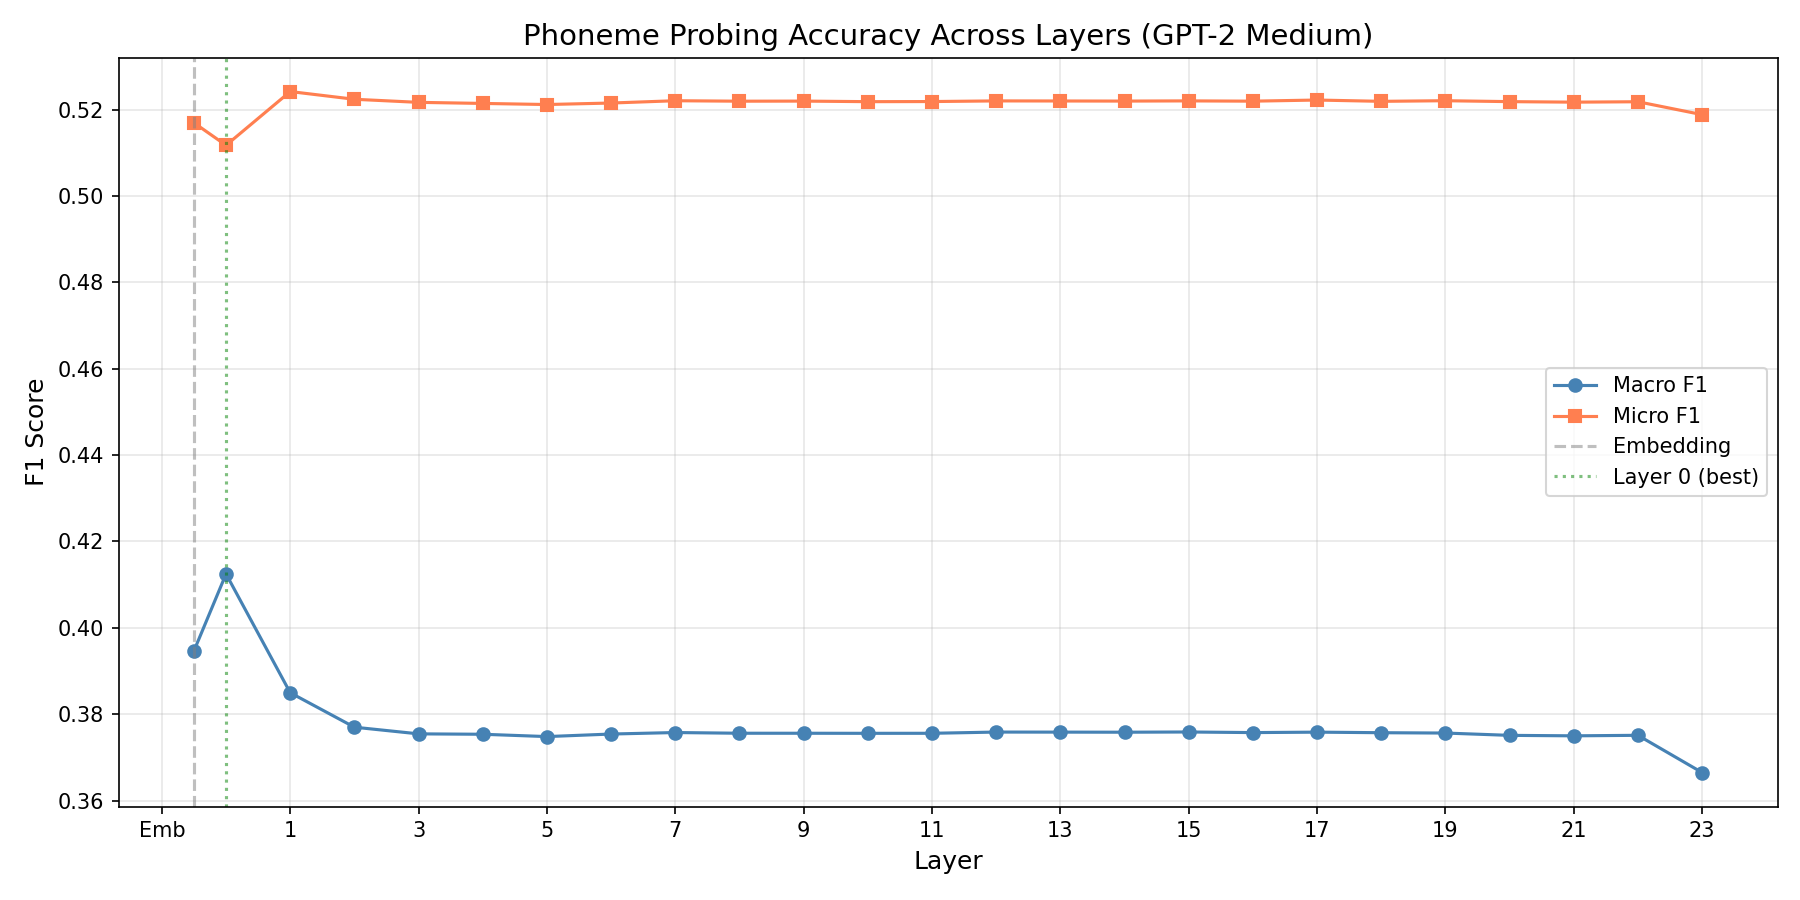
\includegraphics[width=0.95\linewidth]{figures/layer_probing_f1.png}
    \caption{Macro and micro F1 across all 25 layers of \gptmed. Phonetic probe accuracy peaks at layer~0 and remains flat or slightly declining through deeper layers, indicating phonetic information is established early and not built up through the network.}
    \label{fig:layer_probing}
\end{figure}

Performance varies substantially across phonemes.
\Figref{fig:per_phoneme} shows per-phoneme F1 scores at the best layer.
The most accurately predicted phonemes are /\textipa{N}/ (F1 = 0.80), /\textipa{I}/ (0.70), /\textipa{@}/ (0.69), /z/ (0.67), /n/ (0.60), /t/ (0.60), and /k/ (0.60).
However, 47 of 77 phonemes have F1 = 0, almost entirely rare phonemes (aspirated variants, syllabic consonants, infrequent diphthongs) with too few examples in our single-token word set.
Of the 49 phonemes with $\geq$30 occurrences, 30 achieve F1 $>$ 0.1.

\begin{figure}[t]
    \centering
    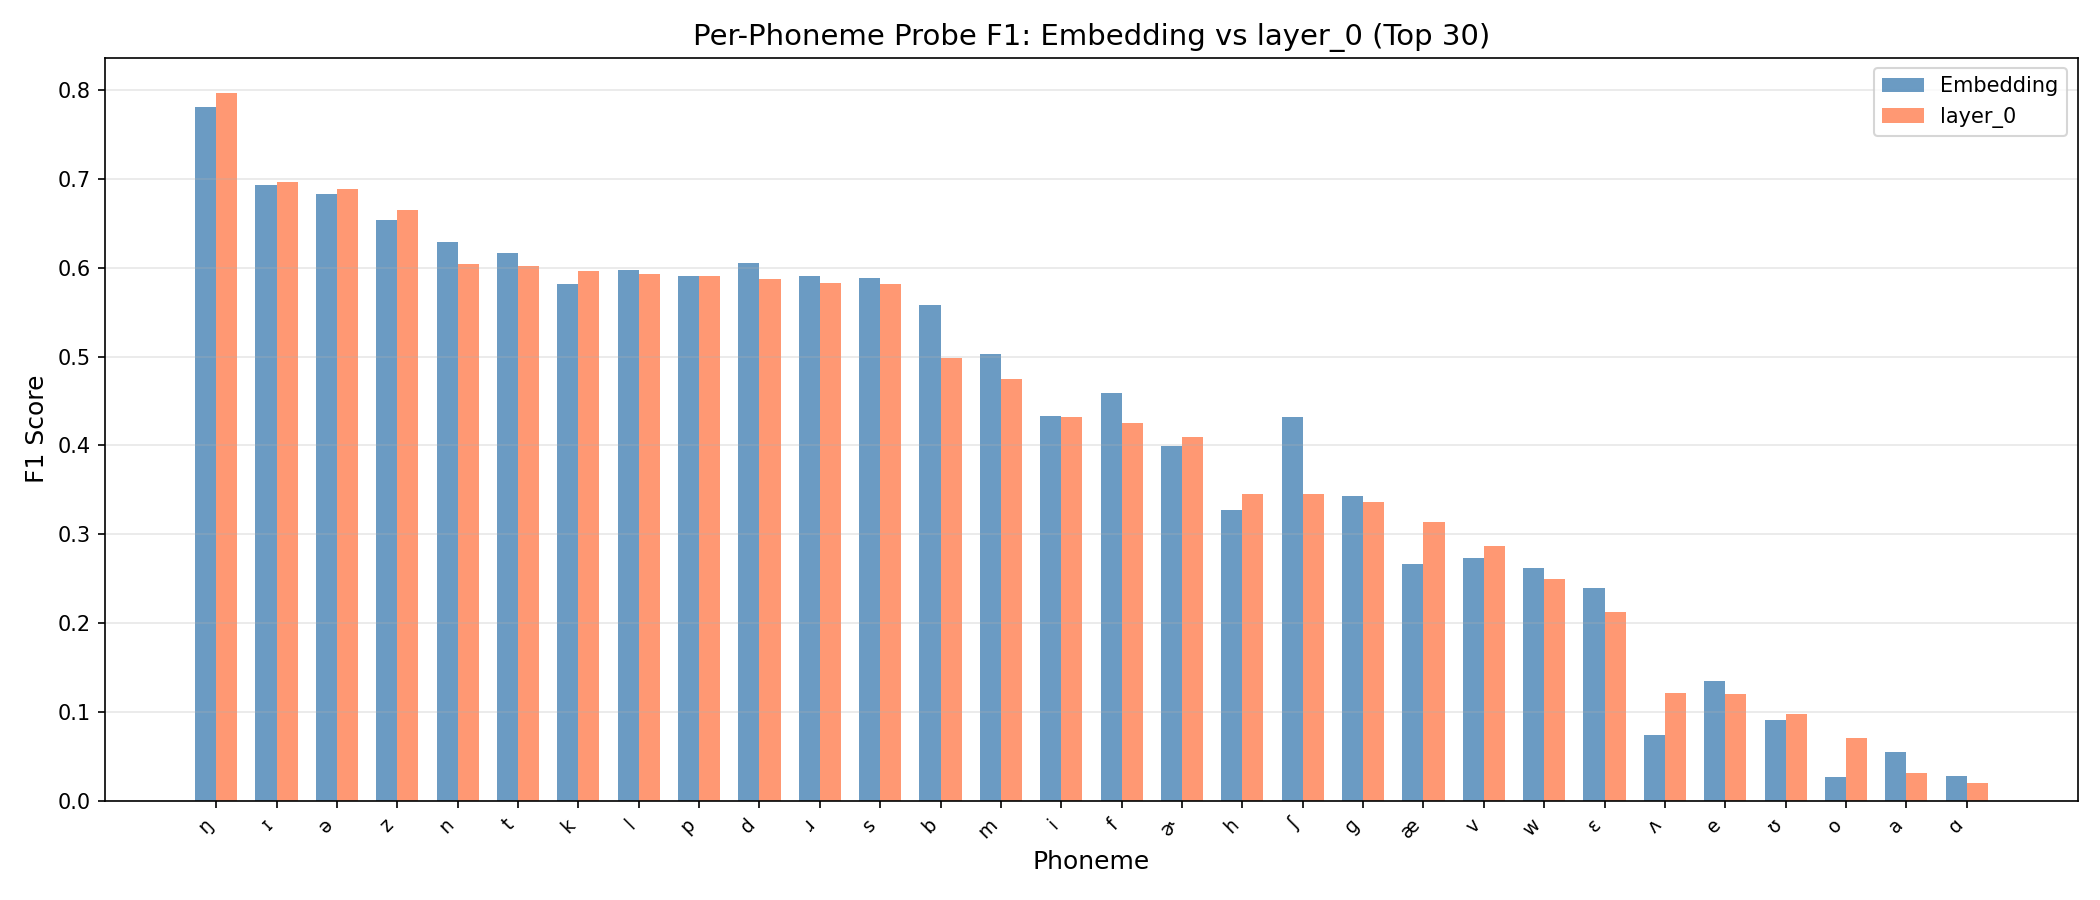
\includegraphics[width=0.95\linewidth]{figures/per_phoneme_f1.png}
    \caption{Per-phoneme F1 scores at the best probing layer (layer~0). Common phonemes like \textipa{N}, \textipa{I}, and \textipa{@} are predicted most accurately, while rare phonemes (aspirated variants, syllabic consonants) have near-zero F1.}
    \label{fig:per_phoneme}
\end{figure}

\subsection{Phoneme Directions: Structured but Not Orthogonal}
\label{sec:geometry}

\begin{table}[t]
    \centering
    \caption{Phoneme direction geometry across layers. Mean $|\text{cos sim}|$ measures alignment between phoneme direction vectors; higher values indicate less orthogonal (more overlapping) representations. The expected value for random directions in $\sR^{1024}$ is 0.025. Silhouette scores test whether phoneme directions cluster by articulatory categories; negative values indicate no clustering.}
    \begin{tabular}{@{}lcccc@{}}
        \toprule
        \textbf{Layer} & \textbf{Mean $|\text{cos}|$} & \textbf{Random} & \textbf{Sil.\ (V/C)} & \textbf{Sil.\ (Manner)} \\
        \midrule
        Embedding & \textbf{0.133} & 0.025 & $-0.032$ & $-0.102$ \\
        Layer 0   & 0.175 & 0.025 & $-0.030$ & $-0.096$ \\
        Layer 11  & 0.270 & 0.025 & $-0.037$ & $-0.131$ \\
        Layer 23  & 0.304 & 0.025 & $-0.039$ & $-0.160$ \\
        \bottomrule
    \end{tabular}
    \label{tab:geometry}
\end{table}

\Tabref{tab:geometry} summarizes the geometry of phoneme direction vectors.
At the embedding layer, the mean pairwise absolute cosine similarity between phoneme directions is 0.133---$5.3\times$ higher than the 0.025 expected for random unit vectors in $\sR^{1024}$.
This confirms that phonemes have distinct but non-random directions: they share significant representational structure rather than occupying independent subspaces.

\Figref{fig:orthogonality} shows how this alignment evolves across layers.
Phoneme directions become \emph{more} aligned in deeper layers (0.133 $\rightarrow$ 0.175 $\rightarrow$ 0.270 $\rightarrow$ 0.304), indicating that the network progressively compresses phonetic variation as it builds semantic representations.
The phonetic manifold contracts rather than expanding through the network.

\begin{figure}[t]
    \centering
    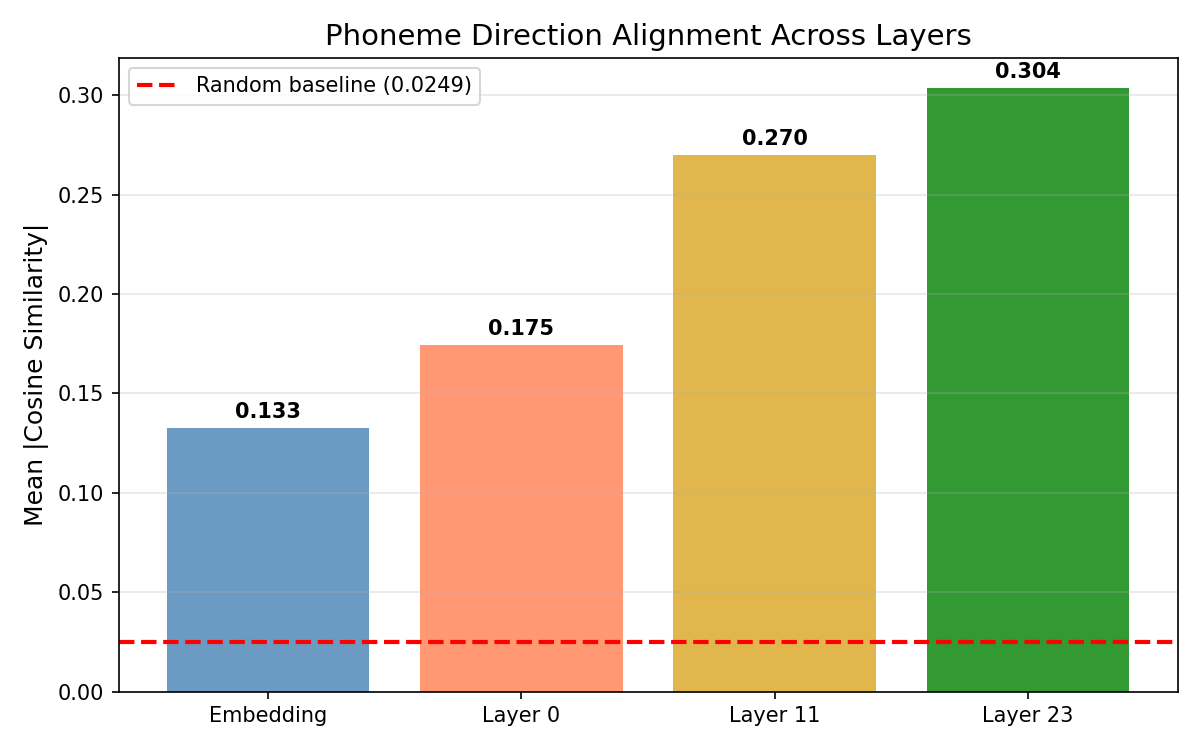
\includegraphics[width=0.95\linewidth]{figures/orthogonality_across_layers.png}
    \caption{Mean absolute cosine similarity between phoneme direction vectors across layers. Phoneme directions become increasingly aligned (less orthogonal) in deeper layers, suggesting phonetic structure is compressed as semantic representations develop. The dashed line shows the expected value for random vectors.}
    \label{fig:orthogonality}
\end{figure}

{\bf Articulatory clustering is absent.}
Silhouette scores for grouping phoneme directions by vowel/consonant ($-0.032$) and manner of articulation ($-0.102$) are consistently negative (\tabref{tab:geometry}), indicating that phoneme directions in \gptmed do \emph{not} organize by traditional articulatory categories.
This diverges from \citet{mclaughlin2025rhyme}, who found organized phonetic structure in the result vectors of phoneme mover heads in \llama.
The distinction is important: articulatory clustering may emerge in specialized attention head outputs rather than in the general residual stream.

{\bf PCA structure.}
\Figref{fig:pca} shows PCA projections of phoneme direction vectors at the embedding layer.
The top five principal components explain 13.1\%, 8.7\%, 8.4\%, 7.0\%, and 6.2\% of the variance respectively.
While vowels and consonants do not form clean clusters, we observe some local structure: nasal consonants group together, and front vowels separate from back vowels along certain axes.

\begin{figure}[t]
    \centering
    \begin{subfigure}[b]{0.32\textwidth}
        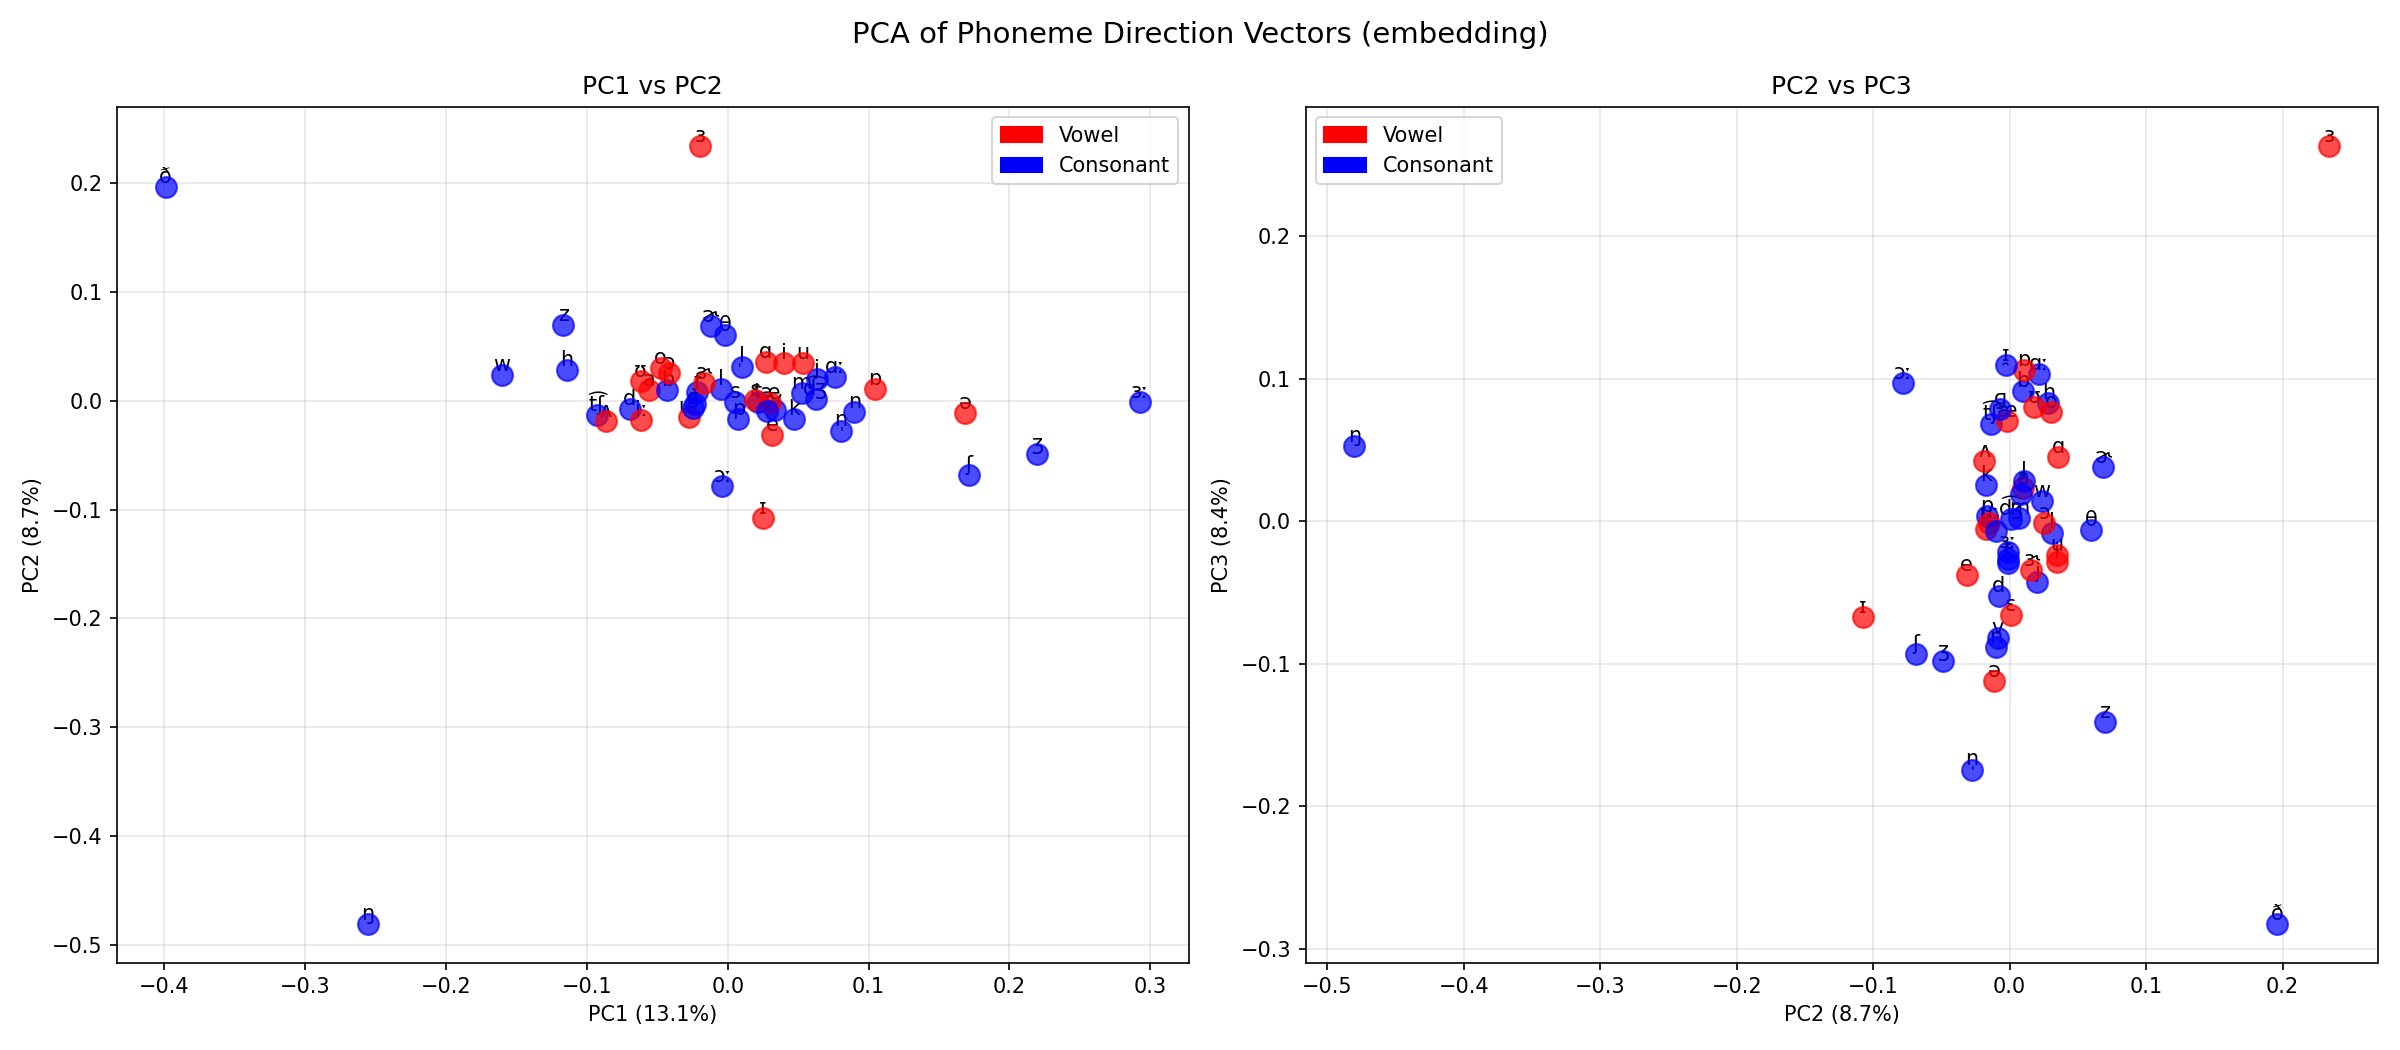
\includegraphics[width=\textwidth]{figures/phoneme_pca_embedding.png}
        \caption{All phonemes}
        \label{fig:pca_all}
    \end{subfigure}
    \begin{subfigure}[b]{0.32\textwidth}
        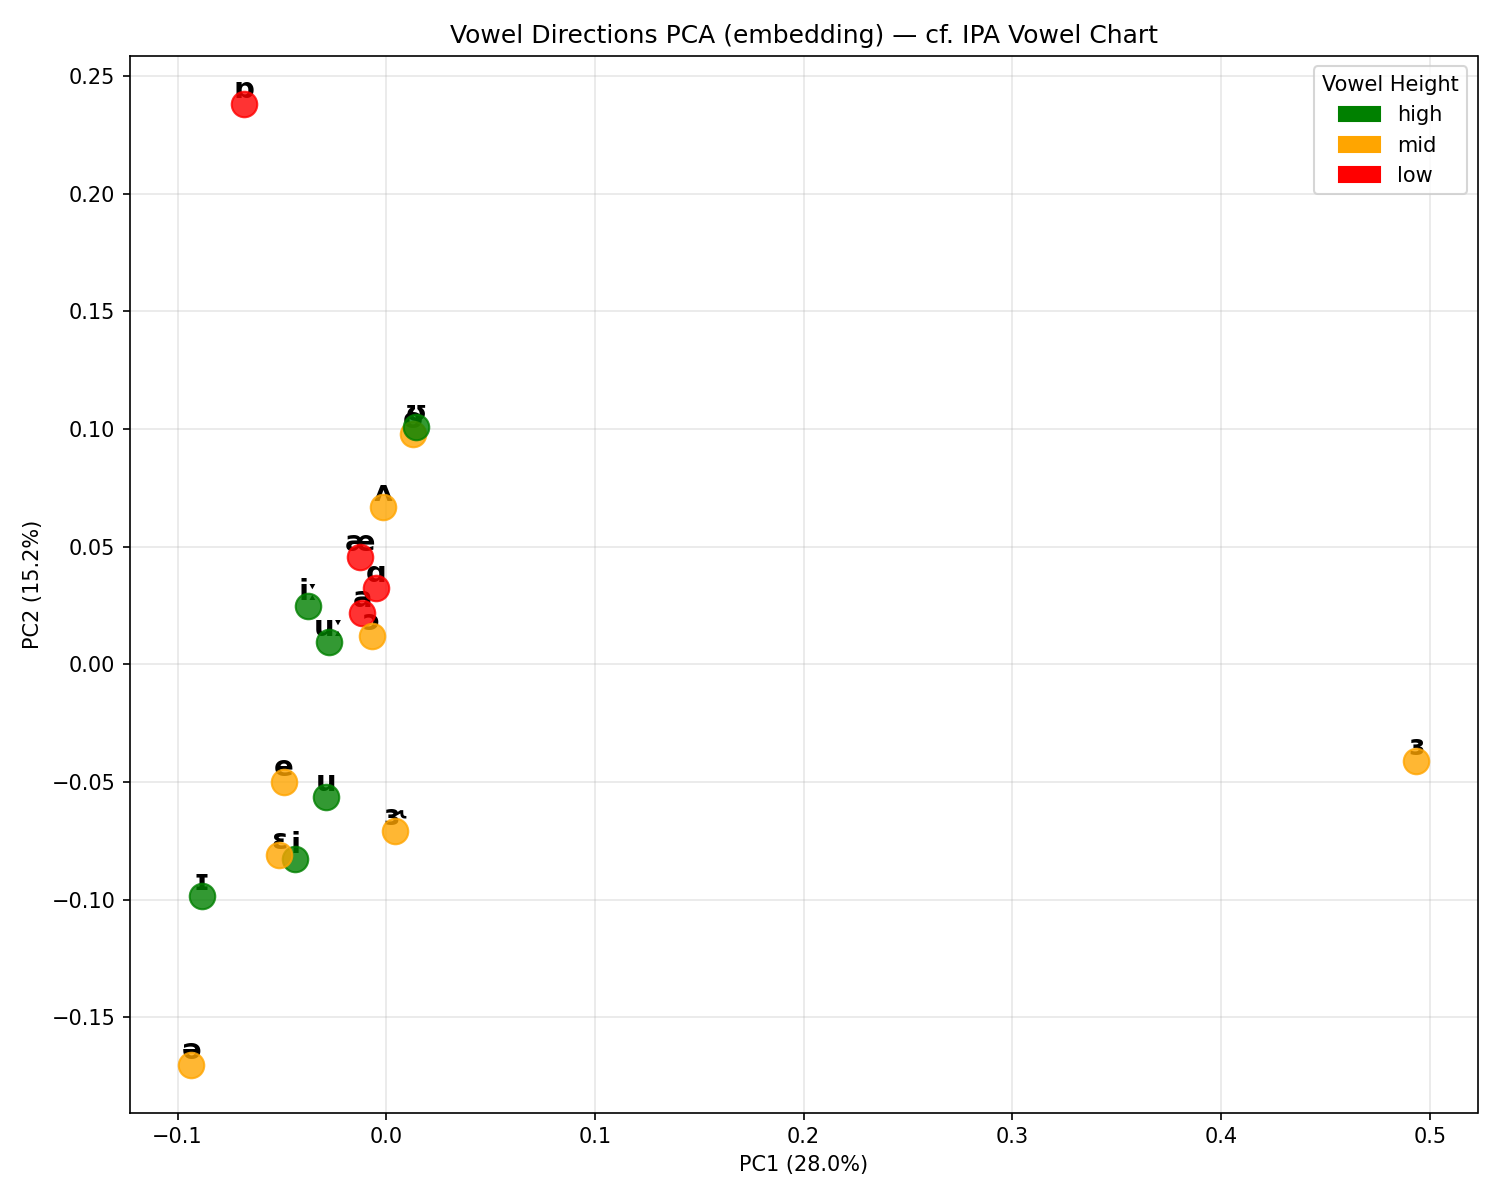
\includegraphics[width=\textwidth]{figures/vowel_chart_embedding.png}
        \caption{Vowels only}
        \label{fig:pca_vowels}
    \end{subfigure}
    \begin{subfigure}[b]{0.32\textwidth}
        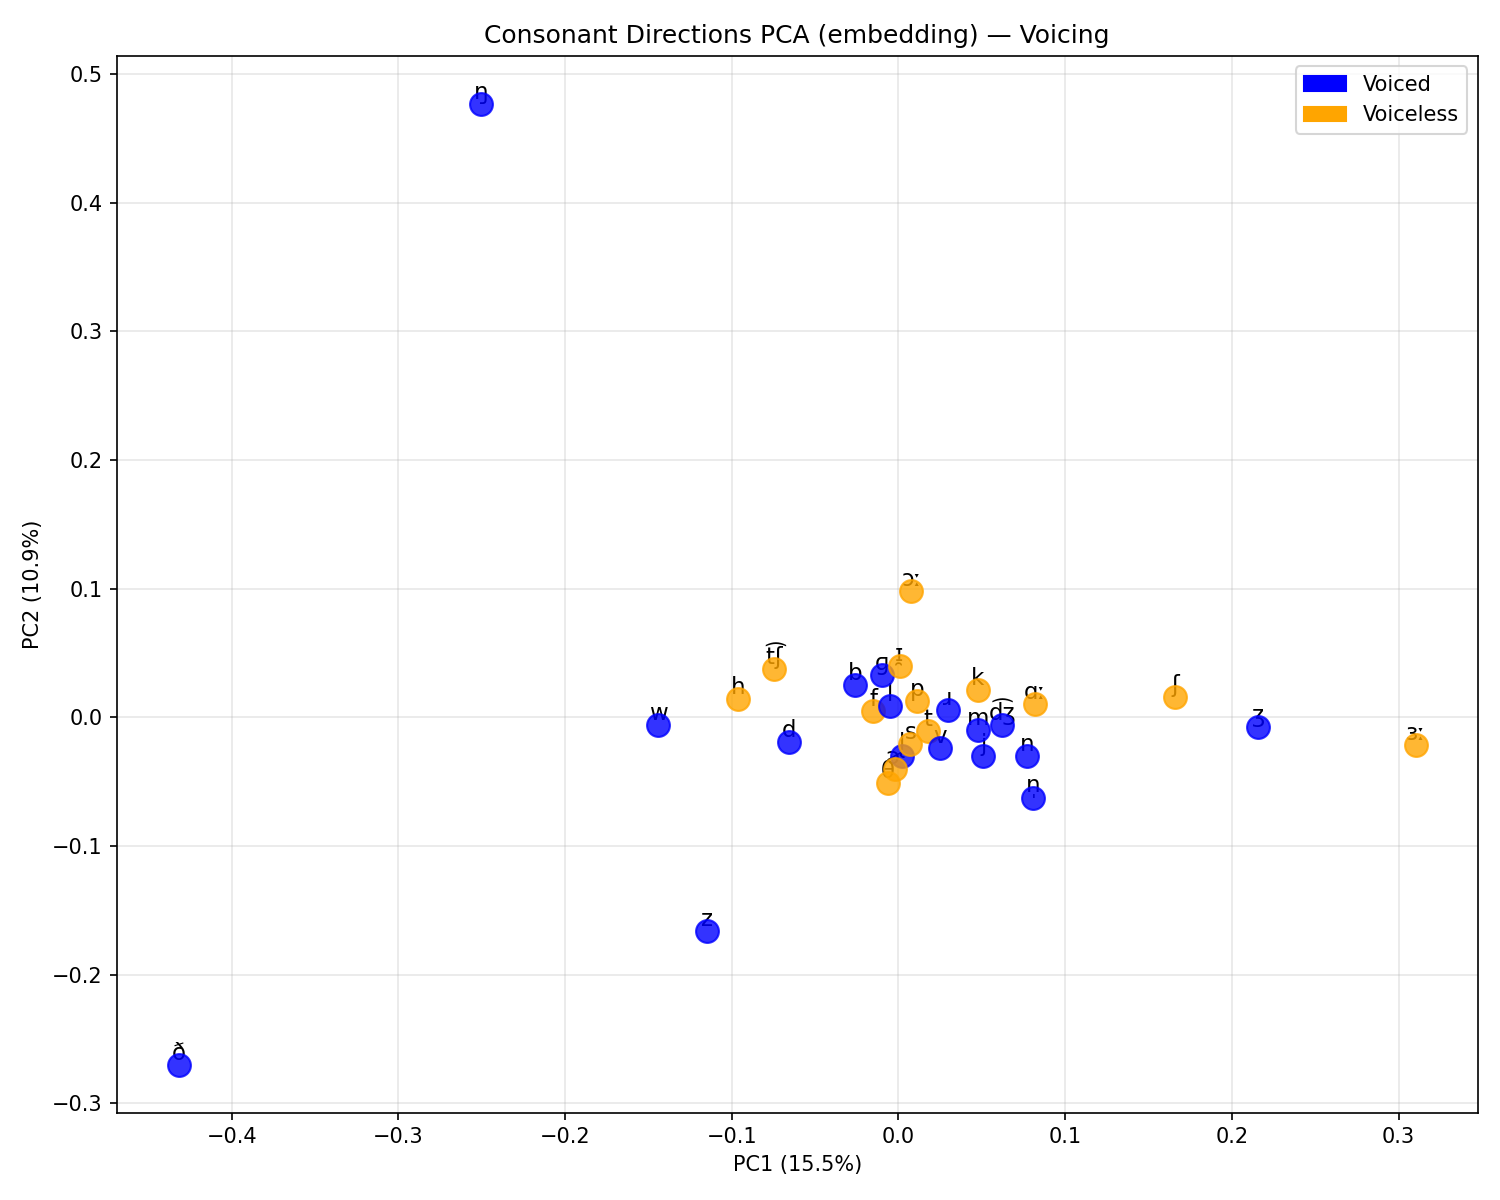
\includegraphics[width=\textwidth]{figures/consonant_voicing_embedding.png}
        \caption{Consonants only}
        \label{fig:pca_consonants}
    \end{subfigure}
    \caption{PCA projections of phoneme direction vectors at the embedding layer. \captiona~All 49 phonemes with $\geq$30 occurrences. \captionb~Vowels show partial separation by backness. \captionc~Consonants show partial separation by voicing.}
    \label{fig:pca}
\end{figure}


\subsection{Context-Dependent Rhyming Reveals Primary-Pronunciation Bias}
\label{sec:context}

\begin{table}[t]
    \centering
    \caption{Context-dependent rhyming accuracy for \gptfour. The model achieves perfect accuracy on standard rhyming but shows a strong bias toward primary pronunciations when handling heteronyms. Best results in \textbf{bold}.}
    \begin{tabular}{@{}lcc@{}}
        \toprule
        \textbf{Test Category} & \textbf{Correct} & \textbf{Accuracy (\%)} \\
        \midrule
        Standard (easy)        & 15/15 & \textbf{100} \\
        Standard (tricky)      & 5/5   & \textbf{100} \\
        \midrule
        Heteronym -- primary   & 11/12 & 92 \\
        Heteronym -- secondary & 7/12  & 58 \\
        \midrule
        \textbf{Overall heteronym} & 18/24 & 75 \\
        \bottomrule
    \end{tabular}
    \label{tab:heteronym}
\end{table}

\Tabref{tab:heteronym} shows rhyming accuracy for \gptfour.
On standard rhyming pairs---including orthographically tricky pairs like ``cough'' and ``off''---the model achieves 100\% accuracy (20/20).
However, heteronyms reveal a systematic asymmetry: 92\% accuracy on primary pronunciations versus only 58\% on secondary pronunciations.

The failure pattern is informative.
\gptfour defaults to the primary pronunciation for ``wind'' ($\rightarrow$ ``pinned'' not ``find''), ``bow'' ($\rightarrow$ ``cow'' not ``show''), ``bass'' ($\rightarrow$ ``class'' not ``face''), ``minute'' ($\rightarrow$ ``in it'' not ``cute''), and ``live'' ($\rightarrow$ ``give'' not ``five''), even when sentence context clearly indicates the secondary pronunciation.
It correctly handles context for ``read,'' ``lead,'' ``tear,'' ``dove,'' ``close,'' and ``refuse.''

This asymmetry is consistent with our probing results: if phonetic information is primarily stored in the static embedding, the model will default to whichever pronunciation dominates in training data.
Overriding this default requires contextual processing that the model performs imperfectly.
